\subsection{Codabench}
{{\footnotesize
\noindent Codabench (successor to CodaLab) is a flexible, easy-to-use, reproducible API platform for hosting AI benchmarks
and code-submission challenges. It supports custom scoring, inverted benchmarks, and scalable public or private queues .


\begin{description}[labelwidth=4cm, labelsep=1em, leftmargin=4cm, itemsep=0.1em, parsep=0em]
  \item[date:] 2022-01-01
  \item[version:] v1.0
  \item[last\_updated:] 2025-03
  \item[expired:] unknown
  \item[valid:] yes
  \item[valid\_date:] 2022-01-01
  \item[url:] \href{https://www.codabench.org/}{https://www.codabench.org/}
  \item[doi:] https://doi.org/10.1016/j.patter.2022.100543
  \item[domain:] General ML; Multiple
  \item[focus:] Open-source platform for organizing reproducible AI benchmarks and competitions
  \item[keywords:]
    - benchmark platform
    - code submission
    - competitions
    - meta-benchmark
  \item[licensing:] https://github.com/codalab/codalab-competitions/wiki/Privacy
  \item[task\_types:]
    - Multiple
  \item[ai\_capability\_measured:]
    - Model reproducibility
    - performance across datasets
  \item[metrics:]
    - Submission count
    - Leaderboard ranking
    - Task-specific metrics
  \item[models:]
    - Arbitrary code submissions
  \item[ml\_motif:]
    - Multiple
  \item[type:] Platform
  \item[ml\_task:]
    - Multiple
  \item[solutions:] Several
  \item[notes:] Hosts 51 public competitions, \textasciitilde{}26 k users, 177 k submissions 

  \item[contact.name:] Isabelle Guyon (Université Paris-Saclay)
  \item[contact.email:] unknown
  \item[results.links.name:] ChatGPT LLM
  \item[fair.reproducible:] Yes
  \item[fair.benchmark\_ready:] Yes
  \item[id:] codabench
  \item[Citations:] \cite{xu-2022}
\end{description}

{\bf Ratings:} ~ \\

\begin{tabular}{p{0.15\textwidth} p{0.07\textwidth} p{0.7\textwidth}}
\hline
Rating & Value & Reason \\
\hline
dataset & 1 & This is a platform for posting benchmarks, not a benchmark in itself.
 \\
documentation & 1 & This is a platform for posting benchmarks, not a benchmark in itself.
 \\
metrics & 1 & This is a platform for posting benchmarks, not a benchmark in itself.
 \\
reference\_solution & 1 & This is a platform for posting benchmarks, not a benchmark in itself.
 \\
software & 1 & This is a platform for posting benchmarks, not a benchmark in itself.
 \\
specification & 1 & This is a platform for posting benchmarks, not a benchmark in itself.
 \\
\hline
\end{tabular}

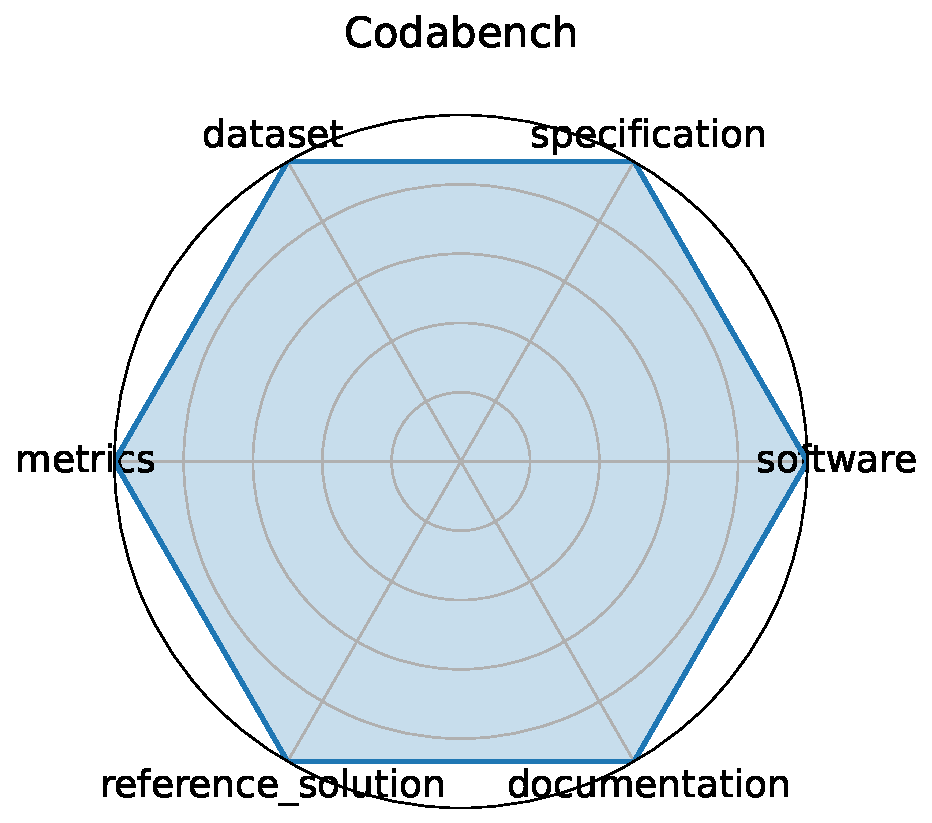
\includegraphics[width=0.2\textwidth]{codabench_radar.pdf}
}}
\clearpage